Antes de hablar de \textbf{Gil} y \textbf{GitHub}. Primero tenemos que comprender el concepto de  control de versiones y porque puede ser útil para tu investigación.
En términos generales, un control de versiones consiste en tomar instantáneas de tus archivos a lo largo del proceso de creación. La mayoría de personas, de hecho, trabajan con algún sistema de control de versiones para gestionar sus archivos. A menudo, el control tiene lugar guardando distintas versiones de un mismo archivo. Por ejemplo, no es raro encontrarnos ante un directorio que contiene los siguientes archivos:\cite{strien_introduccion_2017}

\textbf{midocumento.txt}

\textbf{midocumentoversion2.txt}
   
\textbf{midocumentoconrevisiones.txt}

\textbf{midocumentofinal.txt}

Esta forma de nombrar los archivos puede ser más o menos sistemática. Si añadimos fechas, puede ser un poco más fácil seguir los cambios:

\textbf{midocumento2016-01-06.txt}

\textbf{midocumento2016-01-08.txt}
\newpage
Aunque este método sea un poco más claro, sigue habiendo problemas. En primer lugar, este método no registra o describe qué cambios se han producido entre uno y otro archivo guardado. Pueden ser pequeñas correcciones de erratas, o bien tratarse de la reescritura de pasajes enteros o incluso de una modificación mayor, por ejemplo, de la estructura del documento. Además si quieres revertir alguno de estos cambios, tendrás que averiguar cuándo se hizo el cambio y deshacerlo.\cite{strien_introduccion_2017}

Con un control de versiones se persigue solucionar este tipo de problemas mediante la puesta en marcha de un registro sistemático de cambios en los archivos. A grandes rasgos, puede afirmarse que el control de versiones realiza instantáneas de los archivos a lo largo del tiempo. Estas instantáneas documentan el momento en que fueron tomadas, pero también qué cambios tuvieron lugar entre cada una de ellas, lo cual permite recuperar una versión más antigua de tu archivo. A partir de aquí se abre un sinfín de posibilidades gracias al control de versiones.\cite{strien_introduccion_2017}

 En resumen con un controlador de versiones podemos hacer lo siguiente:

 \begin{itemize}
   \renewcommand{\labelitemi} {\textcolor{red}{$\bigstar$}}
  \item  Rastrear el desarrollo y los cambios de tus documentos
  \item Registrar los cambios que has hecho de una manera que puedas entender posteriormente
  \item Experimentar con versiones distintas de un documento al mismo tiempo que conservas la más antigua
  \item Fusionar dos versiones de un documento y administrar los conflictos existentes entre distintas versiones
  \item Revertir cambios y volver atrás gracias al historial de versiones anteriores de tu documento
 \end{itemize}

 En concreto, el control de versiones es útil para facilitar la colaboración. De hecho, una de las razones que explican el origen del control de cambios es que permitera a varias personas trabajar al mismo tiempo en un proyecto de considerables dimensiones. Para poder hacer esto trabajarermos con GIT y GITHUB\cite{strien_introduccion_2017}

\subsection{¿QUE ES GIT Y GITHUB?}
\subsubsection{GIT}
GIT es un software de control de versiones, su propósito es llevar registro de los cambios en archivos de computadora y coordinar el trabajo que varias personas realizan sobre archivos compartidos (También puedes trabajar solo no hay problema). \cite{noauthor_introduccion_nodate}

\subsubsection {FLOJO DE TRABAJO DE GIT}
 \begin{figure}[H]
    \centering
    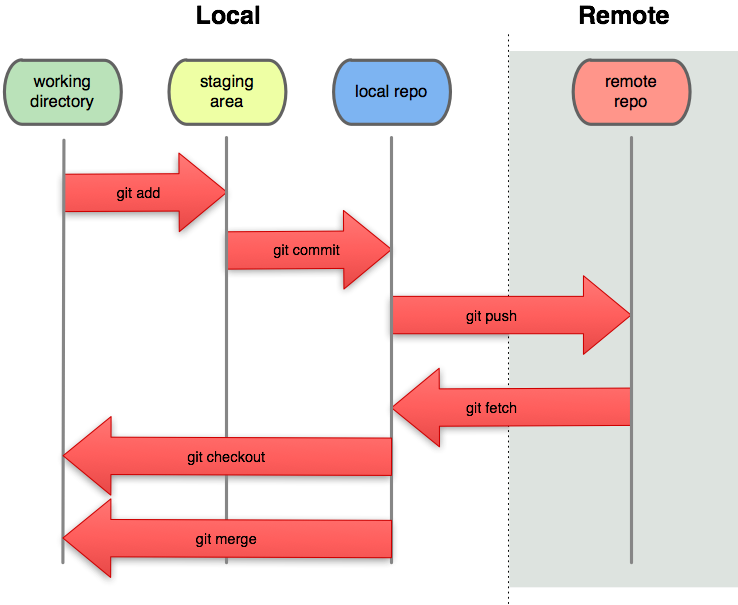
\includegraphics[width=0.6\textwidth]{img/gitflujo.png}
    \caption{Flojo de trabajo GIT}
\end{figure}

\textbf{Tratando de explicar la imagen:} Tenemos nuestro directorio local (una carpeta en nuestro pc) con muchos archivos, Git nos irá registrando los cambios de archivos o códigos cuando nosotros le indiquemos, así podremos viajar en el tiempo retrocediendo cambios o restaurando versiones de código, ya sea en Local o de forma Remota (servidor externo). En la práctica quedará más claro.\cite{noauthor_introduccion_nodate}

\textbf{Página oficial para que descargues este Software: }
\begin{minipage}[c]{0,17 \textwidth}
 \href{https://git-scm.com/}{
 \def\svgwidth{0.9\textwidth}
 \input{IMGSVG/CLICAQUI.pdf_tex}} 
 \end{minipage}\hyperlink{git}{\textcolor{red}{$\looparrowright$URL8$\looparrowleft$}}


 \textbf{Videtutorial de intalacion: }
 \begin{minipage}[c]{0,17 \textwidth}
  \href{https://youtu.be/h9ZH2wFpSUc}{
  \def\svgwidth{0.9\textwidth}
  \input{IMGSVG/VERVIDEO.pdf_tex}} 
  \end{minipage}\hyperlink{videogit}{\textcolor{red}{$\looparrowright$URL9$\looparrowleft$}}



  \textbf{ Tutorial web de intalacion:}
  \begin{minipage}[c]{0,17 \textwidth}
  \href{https://www.mclibre.org/consultar/informatica/lecciones/git-instalacion.html}{
  \def\svgwidth{0.9\textwidth}
  \input{IMGSVG/CLICAQUI.pdf_tex}} 
  \end{minipage}\hyperlink{texgit}{\textcolor{red}{$\looparrowright$URL10$\looparrowleft$}}
  
  \subsubsection{GITHUB}
Es una plataforma de desarrollo colaborativo para alojar proyectos (en la nube) utilizando el sistema de control de versiones Git, Además cuenta con una herramienta muy útil que es GitHub Pages donde podemos publicar nuestros proyectos estáticos (HTML, CSS y JS) gratis.\cite{noauthor_introduccion_nodate}

\textbf{Página oficial para que entres y te registres:}
\begin{minipage}[c]{0,17 \textwidth}
 \href{https://github.com/}{
 \def\svgwidth{0.9\textwidth}
 \input{IMGSVG/CLICAQUI.pdf_tex}} 
 \end{minipage}\hyperlink{github}{\textcolor{red}{$\looparrowright$URL11$\looparrowleft$}}

 \textbf{Tutorial web de registro:}
 \begin{minipage}[c]{0,17 \textwidth}
 \href{https://git-scm.com/book/es/v2/GitHub-Creaci%C3%B3n-y-configuraci%C3%B3n-de-la-cuenta}{
 \def\svgwidth{0.9\textwidth}
 \input{IMGSVG/CLICAQUI.pdf_tex}} 
 \end{minipage}\hyperlink{tutogithubt}{\textcolor{red}{$\looparrowright$URL12$\looparrowleft$}}
 \newpage 




